% cordillera-climate.tex
% ----------------------------------------------------------------------

% Copernicus manuscript
\documentclass[tc, ms]{copernicus}

% Copernicus final print
%\documentclass[tc]{copernicus}

% Copernicus discussion paper
%\documentclass[tcd, hvmath]{copernicus_discussions}

% Copernicus-like latex2rtf compatible
%% copernicus_rtf.tex
% ------------------

% Base class and packages
\documentclass{article}
\usepackage{color}
\usepackage{geometry}
\usepackage{graphicx}
\usepackage{setspace}
\onehalfspacing

% Replacements for bibtex commands
\newcommand{\citep}[1]{(\textcolor{blue}{#1})}
\newcommand{\citet}[1]{\textcolor{blue}{#1}}

% Replacements for Copernicus commands
\newcommand{\introduction}[0]{\section{Introduction}}
\newcommand{\conclusions}[0]{\section{Conclusions}}
\newcommand{\tophline}[0]{\hline}
\newcommand{\middlehline}[0]{\hline}
\newcommand{\bottomhline}[0]{\hline}
\newcommand{\unit}[1]{\ensuremath{\mathrm{#1}}}
\newcommand{\degree}[0]{\ensuremath{^{\circ}}}

% Ignore other Copernicus commands
\newcommand{\runningtitle}[1]{}
\newcommand{\runningauthor}[1]{}
\newcommand{\received}[1]{}
\newcommand{\correspondence}[1]{}
\newcommand{\pubdiscuss}[1]{}
\newcommand{\revised}[1]{}
\newcommand{\accepted}[1]{}
\newcommand{\published}[1]{}



% Coloured hyperlinks
\usepackage[colorlinks,citecolor=blue]{hyperref}

% Recognize utf-8 special characters
\usepackage[T1]{fontenc}
\usepackage[utf8]{inputenc}

% Set figures repository
\graphicspath{{figures/}}

% ----------------------------------------------------------------------
\begin{document}
% ----------------------------------------------------------------------

% Title
\title{The effect of climate forcing on numerical simulations of the Cordilleran Ice Sheet at the Last Glacial Maximum}
\runningtitle{Climate forcing for Cordilleran ice sheet simulations}

% Authors
\author[1]{Julien Seguinot}
\author[2]{Constantine Khroulev}
\author[3]{Irina Rogozhina}
\author[1]{Arjen P. Stroeven}
\author[1]{Qiong Zhang}
\runningauthor{J. Seguinot et al.}
\correspondence{J. Seguinot\\ (julien.seguinot@natgeo.su.se)}

% Affiliations
\affil[1]{Department of Physical Geography and Quaternary Geology, Stockholm University, Stockholm, Sweden}
\affil[2]{Geophysical Institute, University of Alaska Fairbanks, Fairbanks, AK, USA}
\affil[3]{Helmholtz Centre Potsdam, GFZ German Research Centre for Geosciences, Potsdam, Germany}

% For Copernicus
\received{}
\pubdiscuss{}
\revised{}
\accepted{}
\published{}

% Title
\maketitle

% Sections
% section/abstract.tex
% ----------------------------------------------------------------------

\begin{abstract}
We present an ensemble of numerical simulations of the Cordilleran Ice Sheet during the Last Glacial Maximum performed with the Parallel Ice Sheet Model (PISM), using temperature offsets from present-day climatologies from five different datasets. Monthly mean surface air temperature and precipitation from the NCEP/NCAR reanalysis, the Climate Forecast System Reanalysis, the ERA-Interim reanalysis and the North American Regional Reanalysis are used to compute surface mass balance by using a positive degree-day model. Modelled ice sheet outlines and volumes appear highly sensitive to the choice of climate forcing. We assess model performance against a reconstruction of the ice margin at the Last Glacial Maximum in continental regions of northern Yukon Territory and interior Alaska. The best match between model output and the reconstructed ice margin is obtained using climate forcing from the North American Regional Reanalysis, which is a regional climate reanalysis with the highest resolution.
\irina{Maybe more on conclusions.}
\end{abstract}

% section/intro.tex
% ----------------------------------------------------------------------
\introduction
\label{sec:intro}
% ----------------------------------------------------------------------

At the Last Glacial Maximum (LGM), glaciers of a size comparable to the present Greenland and Antarctic ice sheets covered parts of Northern America (Laurentide, Cordilleran and Innuitian ice sheets) and Northern Eurasia (Fennoscandian Ice Sheet). Numerical modelling of these former ice masses allows for a comparison between glaciological theories embedded in the models and geomorphological traces underpinning palaeo-glaciological reconstructions. Yet, a major obstacle in this exercise resides in large uncertainties concerning climate forcing, typically temperature and precipitation data, needed by numerical glacier models \citep{hebeler-etal-2008}. This includes uncertainty in representation of Earth's present climate in regions of poor station coverage, and even larger uncertainty concerning accurate reconstructions of past climate change.

Arguably the most physically sound way to force an ice sheet model in the past is to couple it with a General Circulation Model (GCM) \citep{yoshimori-etal-2001,calov-etal-2002,abeouchi-etal-2007,charbit-etal-2013}. However the computational demand of GCMs is such that only models of intermediate complexity can run on the time-scales of tens of thousands of years characteristic of ice sheet growth and decay.

Climatologies obtained from uncoupled GCM palaeo-climate simulations such as produced within the PMIP project \citep{joussaume-taylor-1995} provide a more accurate representation of past climate and are commonly used to force ice sheet models. Because such climatologies are only available for specific periods of time, this method requires either an assumption of steady-state \citep{huybrechts-tsiobbel-1996}, or interpolation through time between climatologies from different periods, which can be linear \citep{charbit-etal-2002}, or modulated by a ``glacial index'' weighting function derived from ice core $\delta^{18}$\,O records \citep{marshall-clarke-1999,tarasov-peltier-2004,zweck-huybrechts-2005,gregoire-etal-2012}. An important drawback in this approach is that palaeo-climate simulations themselves rely on global ice sheet reconstructions such as the ICE-4G \citep{peltier-1994} for their surface topographic boundary condition. This exerts indirect influence on subsequently modelled ice sheet geometries, whose spatial extent tends to conform to these reconstructions.
\julien[noline]{Should I include references not covering the Cordilleran Ice Sheet?}

The other side of the coin is that avoiding this circular dependence unfortunately goes hand-in-hand with a need for simplifying assumptions on Earth's past climate. They include energy balance modelling approaches \citep{tarasov-peltier-1997} and geographic parametrizations of surface mass balance \citep{robert-1991} or climate forcing \citep{johnson-fastook-2002}. Standing on a middle ground, temperature offset methods \citep{greve-etal-1999,bintanja-etal-2005} make use of the high level of detail available in present climate datasets such as gridded observation datasets, GCM output or reanalyses, while using simplifying representations of past climate deviations from this present state.

Here, we propose to address some of the uncertainties concerning climate forcing of numerical glacier models by evaluating their responses, in terms of glacier extent, to inputs from several climate datasets. Few studies of this kind are presently available. \citet{quiquet-etal-2012} assessed the sensitivity of a Greenland ice sheet model to various atmospheric forcing, including a regional parametrization \citep{fausto-etal-2009}, output from several GCMs and a climate reanalysis. \citet{rodgers-etal-2004} and \citet{charbit-etal-2007} tested the sensitivity of a model of the Northern Hemisphere ice sheets to different PMIP LGM simulations. Here, to limit degrees of freedom in our model, and obtain results independent of palaeo-ice sheet reconstructions such as the ICE-4G, we use a simple temperature offset approach similar to \citep{greve-etal-1999} and \citet{bintanja-etal-2005} and assess ice sheet model sensitivity to the choice of present-day climate data. Rather than using GCM output, we force our model with climate reanalysis data, which include observational information through data assimilation \citep{bengtsson-etal-2007}. Furthermore, we focus our study regionally on the former Cordilleran Ice Sheet in Northern America.

The Cordilleran Ice Sheet (Fig.~\ref{fig:locmap}) covered an area that presently experiences strong regional variations in climate. In a numerical modelling perspective, it is one of the least studied palaeo-ice sheets of the Northern Hemisphere, despite the fact that significant geomorphological data is available to constrain its extent \citep{jackson-clague-1991,dukrodkin-1999,kaufman-manley-2004,kleman-etal-2010,margold-etal-2011}. Although the Cordilleran Ice Sheet was not the primary target of these simulations, it has previously been modelled as part of efforts to model ice sheets in North America \citep{marshall-clarke-1999,calov-etal-2002,tarasov-peltier-1997,tarasov-peltier-2004,gregoire-etal-2012}, the Northern Hemisphere \citep{huybrechts-tsiobbel-1996,greve-etal-1999,charbit-etal-2002,charbit-etal-2007,charbit-etal-2013,johnson-fastook-2002,rodgers-etal-2004,bintanja-etal-2005,zweck-huybrechts-2005,abeouchi-etal-2007} or world-wide \citep{yoshimori-etal-2001}. While these studies reproduce the magnitude of North American glaciation at LGM reasonably well, there exists a tendency in the simulations that are independent of ice sheet reconstructions such as the ICE-4G to predict excessive ice cover in parts of northern Yukon Territory and continental Alaska that have remained ice-free throughout the Pleistocene \citep{dukrodkin-1999,kaufman-manley-2004}.

Here we use a PISM, a Parallel Ice Sheet Model \citep{web:pism}\julien{Citation recommended by \url{http://www.pism-docs.org/wiki/doku.php?id=citing_pism}}, to simulate the extent and thickness of Cordilleran Ice Sheet at the LGM. We force our model with multiple climate datasets and compare our results to the mapped LGM ice sheet margin from \citet{dyke-2004}. To our knowledge, this is the first modelling study that specifically focuses on the Cordilleran Ice Sheet since the one by \citet{robert-1991}. While the modelling domain of \citet{robert-1991} covered only the southern part of the ice sheet, our model also includes higher resolution and an improved treatment of ice thermodynamics and bedrock response following the large advances made in ice sheet modelling since then. Model set-up is presented in section~\ref{sec:model} and climate forcing in section~\ref{sec:climate}. Results are exposed in section~\ref{sec:results} and discussed in section~\ref{sec:discussion}.


% ----------------------------------------------------------------------
\section{Model setup}
\label{sec:setup}
% ----------------------------------------------------------------------



% ----------------------------------------------------------------------
\section{Climate forcing}
\label{sec:climate}
% ----------------------------------------------------------------------

\subsection{Observation data}

WorldClim \citep{data:worldclim} is a high resolution climate dataset interpolated between from weather station data over global land areas. The interpolation uses 30\,arc\,s aggregated, hole-filled SRTM\needref data \todo{check WorldClim methods}, which provides a resolution much higher than attained by general circulation models.

However, the density of weather stations used by WorldClim in the Northern American Cordillera is highly inhomogeneous, and if good coverage exists in the southern parts of our modelling domain, several hundred kilometers can separate nearby stations in the north \citep{data:worldclim}.

A second drawback of the dataset in an ice sheet modelling view is the lack of data on marine surfaces, particularly on the Pacific continental shelf where glaciers have advanced during the last glacial cycle\needref.

% ----------------------------------------------------------------------

\subsection{Reanalysis data}

In addition to the WorldClim data, we use three global and one regional climate reanalysis to force the ice sheet model. Monthly climatologies from the NCEP/NCAR reanalysis\needref and the North American Regional Reanalysis (NARR)\needref were obtained from the NOAA ESRL's PSD website\needref, and monthly climatologies from the ERA-Interim\needref and Climate System Forecast Reanalyses (CFSR)\needref were computed from their monthly mean timeseries. As a mixed product of observation and circulation model, we believe that reanalysis may perform best in poorly monitored regions such as the northernmost American Cordillera. Additional information on the data used is gatherd in table \ref{tab:reanalyses}\todo{fill the table}.

\begin{table}[t]
	\caption{Characteristic of reanalysis data used as a forcing for the ice sheet model.}
	\label{tab:reanalyses}
	\vskip4mm
	\centering
	\begin{tabular}{lllll}
		\tophline
		Reanalysis& coverage& time period&  resolution& reference\\
		\middlehline
		NCEP/NCAR&  global&   1981 -- 2010& ??& ??\\
		ERA-Interim&global&   1979 -- 2011& ??& ??\\
		CFSR&       global&   1979 -- 2010& ??& ??\\
		NARR&       global&   1979 -- 2000& ??& ??\\
		\bottomhline
	\end{tabular}
\end{table}

% ----------------------------------------------------------------------

\subsection{Cordilleran climates}

\begin{figure}[t]
	\vspace*{2mm}
	\begin{center}
		\includegraphics[width=13cm]{cordillera-climate-temp}
	\end{center}
	\caption{Summer temperature maps from the five datasets used in this study and winter temperature map from the WorldClim dataset.}
	\label{fig:temp}
\end{figure}

Figure~\ref{fig:temp} shows the spatial distribution of summer (JJA) air surface temperatures from the five climate datasets used in the study, and winter (DJF) air surface temperatures from the WorldClim interpolated observation data. Summer temperatures are most relevant to the glacier model as they drive summer melt.

As can be expected, temperatures decrease with latitude, and regions further inland experience colder winters. It should be noted that the temperature gradient is much stronger in the winter than it is in the summer, and that at low elevations, temperatures get well above zero during the summer months in the entire modelling domain. In other words, there is a strong seasonality contrast beween coastal and inland regions, and regions where mean annual temperatures are well below freezing do experience warm summers.

\begin{figure}[t]
	\vspace*{2mm}
	\begin{center}
		\includegraphics[width=13cm]{cordillera-climate-prec}
	\end{center}
	\caption{Winter precipitation rate maps from the five datasets used in this study and summer precipitation map from the WorldClim dataset.}
	\label{fig:prec}
\end{figure}

Figure~\ref{fig:prec} shows the spatial distribution of winter (DJF) precipitation rates from the five climate datasets used in the study, and summer (JJA) precipitation rates from the WorldClim interpolated observation data. Winter precipitation is most relevant to the glacier model as it drives winter accumulation.

Once again expectedly, coastal regions recieve much more precipitation than inland ones due to the unborken topographical barrier of the Boundary Ranges / Coast Mountains / Cascadia. It should be noted that from a glacier mass-balance view, this contrast is made even stronger by the difference of timing of the precipitation peak through the year. Although coastal regions experience most precipitation in the accumulation season, inland regions experience dry winters and most of the precipitation falls as rain during the summer months.

In regions like Northern Yukon and Alaska, dry winters and warm summers prevent snow accumulation and glacial inception despite of mean annual temperatures being well below zero at present. In order to account for these strong gradients in seasonality, we use monthly means to drive the ice sheet model. Previous runs made with mean annual temperature and precipitation forcing and not presented here lead to unrealistic ice cover in Northern Yukon and Alaska even under present-day climate while leaving the Coast Mountains free of ice.

% ----------------------------------------------------------------------

\subsection{Preprocessing and lapse-rate corrections}

Air surface temperature and precipitation rates from the NCEP/NCAR reanalysis, the ERA-Interim reanalysis, the CFSR, the NARR and WorldClim data were reprojected to Canadian Atlas Lambert (EPSG code XXXX\todo{add EPSG code}) conformal conic projection. The data were bilinearly interpolated to the model resolution of 10\,km, which is not shown by figures~\ref{fig:temp} and~\ref{fig:prec}.

For the WorldClim data, data holes in oceanic areas were filled by a nearest-neighbour extrapolation to allow ice to extend to these regions.

For the CFSR, an alternative forcing was prepared by smoothing the precipitation fields to avoid artifacts seen in figure~\ref{fig:prec}. This was done by averaging data locally in a circular neighbourhood of 7 pixels in diameter prior to reprojection. However the effect of smoothin the precipitation field is very limited as we will see further. All the preprocessing steps were made in GRASS~GIS using scripts made available on the first author's website.

\begin{figure}[t]
	\vspace*{2mm}
	\begin{center}
		\includegraphics[width=13cm]{cordillera-climate-topo}
	\end{center}
	\caption{Reference topography used for temperature lapse-rate corrections from the five climate datasets used in the study and ETOPO1 topography used as basal condition for the ice flow model.}
	\label{fig:topo}
\end{figure}

Throughout the simulation, the numerical model dynamically applies temperature lapse-rate corrections that account for both differences between the climate reference topography and the ice flow model topography, and the thickness of overlying ice thickness. The reference topography from the five forcing datasets as well as the ETOPO1\citep{data:etopo1} topography used to force the ice flow model are shown in figure~\ref{fig:topo}. A lapse-rate of 6\unit{\degree C\,km^{-1}} was used in all simulations. No lapse-rate corrections are applied to precipitation rate.



% ----------------------------------------------------------------------
\section{Results}
\label{sec:results}
% ----------------------------------------------------------------------

Using climate forcing from WordClim data and the NCEP/NCAR, ERA-Iterim, CFSR and NARR reanalyses described in section~\ref{sec:climate} and the ice sheet model described in section~\ref{sec:model}, we run simulations of glacial inception and growth of the Cordilleran ice sheet using different temperature offsets.

\begin{figure}[t]
	\vspace*{2mm}
	\begin{center}
		\includegraphics[width=13cm]{cordillera-climate-cool06}
	\end{center}
	\todo[inline]{Change panel order to match climate section}
	\caption{Ice surface topography (black contours every 1000\,m) and velocity (\unit{m\,yr^{-1}}) after 10\,kyr under a climate 6\degC colder than present for each climate forcing.}
	\label{fig:cool06}
\end{figure}

Figure~\ref{fig:cool06} shows the effect of a 6\degC temperature offset on the six different climate forcings. It apperas that the magnitude of glaciation differs highly between forcing datasets. NCEP/NCAR and CFSR forcings produce large ice sheets covering parts of Yukon and Alaska which are thought to have remained unglaciated for at least several glacial cycles. \needref The smoothing of CFSR precipitation has limited effect on the resulting ice sheet geometry. The WorldClim forcing results to a glaciation mode limited to major mountain ranges, whereas ERA-Interim and NARR produce medium-sized ice sheets with a difference in shape.

\begin{figure}[t]
	\vspace*{2mm}
	\begin{center}
		\includegraphics[width=13cm]{cordillera-climate-extent}
	\end{center}
	\todo[inline]{Change panel order to match climate section}
	\qiong[inline]{Move ticks on the colorbar. The 1 is confusing.}
	\caption{Extent of ice cover after 10\,kyr as a function of applied temperature offsets for each climate forcing.}
	\label{fig:extent}
\end{figure}

As we aim to model an ice sheet approaching LGM size, yet do not know how cold was the climate shaping it, we apply temperature offsets ranging from 2 to 9\degC for each climate forcing. Figure~\ref{fig:extent} shows the extent of ice cover at the end of each of theses 40~simulations, grouped by climate forcing. Again it is visible that different forcings lead to very different final ice cover, generally. Notably, for the lowest temperature offset of 2\degC, NCAR and CFSR simulatinos lead to a significant ice-sheet, whereas WorldClim, NARR and ERAI produce mountain ice caps, not more extensive than present for WorldClim. It should be noted that several of the NCAR and CFSR simulations producve oversised ice-sheets whose extent is primirily bounded by the model domain boundary conditions rather than any physical process. Where different climate forcings lead to similar ice sheet sizes, differences in pattern can be noted. For instance ERAI ice seets appear more northernly-centered than NARR ice sheets.

\begin{figure}[t]
	\vspace*{2mm}
	\begin{center}
		\includegraphics[width=9cm]{cordillera-climate-ivolarea}
	\end{center}
	\todo[inline]{Use black-and-white-proof markers}
	\todo[inline]{Highlight the ``best'' runs.}
	\caption{Total ice volume and glaciated area after 10\,kyr as a function of temperature offset and climate forcing.}
	\label{fig:ivolarea}
\end{figure}

Figure~\ref{fig:ivolarea} shows the final ice volume and glaciated area at the end of each of the 48~simulations. Differences in ice sheet size can be quantified. ERAI and NARR lead to similar ice volumes and glaciated areas, yet patterns are different as shown by Figure~\ref{fig:extent}.

\begin{figure}[t]
	\vspace*{2mm}
	\begin{center}
		\includegraphics[width=13cm]{cordillera-climate-best}
	\end{center}
	\todo[inline]{Change panel order to match climate section}
	\caption{Ice surface topography (black contours every 1000\,m) and velocity (\unit{m\,yr^{-1}}) after 10\,kyr using temperature offsets that lead to similar areas of ice cover for each climate forcing.}
	\label{fig:best}
\end{figure}

To be able to compare runs of similar magnitudes, and as we consider temperature offset as an unknown in this study, we select for each climate forcing the simulation that lead to most realistic results in terms of glaciated area. This was done by using the LGM extent countour from \needref shown in Figure~\ref{fig:locmap}, which covers an area of XXX \todo{do the maths}. These so called ``best'' runs are presented in Figure~\ref{fig:best} along with the temperature offset values associated.



% ----------------------------------------------------------------------
\section{Discussion}
\label{sec:discussion}
% ----------------------------------------------------------------------

\emph{Coming soon...}


% section/concl.tex
% ----------------------------------------------------------------------
\conclusions
\label{sec:concl}
% ----------------------------------------------------------------------

Our study shows a strong dependency of ice sheet model results on the choice of climate forcing data. For three of the four reanalysis datasets used, precipitation rate, over surface air temperature, causes much of the discrepancy between modelled ice sheet outlines and volumes. Furthermore, the spatial resolution of input data appears critical for providing the ice sheet model with an accurate precipitation field, confirming results obtained by \citet{quiquet-etal-2012} from various GCM forcing over the Greenland Ice Sheet.

For the Cordilleran Ice Sheet, we achieve the best fit to the mapped LGM margin by \citet{dyke-2004} using climate forcing from the high-resolution interpolated observational data WorldClim \citep{data:worldclim} and the North American Regional Reanalysis \citep[NARR;][]{data:narr}. The latter dataset is preferable in our case due to the lack of WorldClim data offshore. Climate forcing from CFSR and the NCEP/NCAR reanalysis produces largely oversized ice sheets due to too high precipitation rates, and in the second case, too low surface air temperature. The ERA-Interim data used in this study produces more reasonable results, but it may be too coarse to accurately resolve the spatial distribution of orographic precipitation associated with the rugged topography of the northern American Cordillera, resulting in a misplaced ice cover in regard to geomorphological data. Therefore, we retain NARR data for forcing future simulations of the Cordilleran Ice Sheet.

One must keep in mind, however, that these results are biased by our choices of ice-sheet model (PISM), surface mass balance (PDD) model, study area (the Cordilleran Ice Sheet), and more importantly palaeo-climate representation (temperature offsets). At LGM, it is most likely that the presence of ice sheets significantly affected circulation patterns and distribution of precipitation. At the cost of greater computational expense, a more accurate representation of palaeo-climate may allow for a better fit between model results and the mapped LGM margin.


% Acknowledgements
\begin{acknowledgements}
We thank Ed Bueler and Andy Aschwanden for providing constant support on PISM and patiently answering our questions on the code internals, Laurent Brodeau and Soon-Heum Ko for assistance concerning software installations on supercomputing resources, and all PISM authors for providing the model open-source. This work was supported by the Swedish Research Council (VR) grant \#2008-3449 to A. P. Stroeven and by NASA grant \#NNX13AM16G to E. Bueler. Computer resources were provided by the Swedish National Infrastructure for Computing (SNIC) allocation \#2013/1-145 to A. P. Stroeven at the National Supercomputing Center (NSC). 

% Author contributions
\textit{Author contributions.}
J. Seguinot ran the simulations and wrote most of the paper; C. Khroulev implemented necessary code changes in PISM; I. Rogozhina helped with model set-up and experiment design; A. P. Stroeven initiated the Cordilleran Ice Sheet modelling project; and Q. Zhang prepared some of the forcing data. All authors contributed to paper writing.
\end{acknowledgements}

% References
\bibliographystyle{copernicus}
\bibliography{references}

% Floats
\newpage
% floats/tables.tex

% tab:reanalyses
\begin{table*}[t]
	\caption{Characteristic of reanalysis climatologies used to force the ice sheet model.}
	\label{tab:reanalyses}
	\vskip4mm
	\centering
	\begin{tabular}{lllll}
		\tophline
		Reanalysis& Spatial coverage& Averaging period& Resolution& Description\\
		\middlehline
		NCEP/NCAR&  global&     1981 -- 2010& 1.875\degree& \citet{data:ncar}\\
		ERA-Interim&global&     1979 -- 2011& 1.000\degree& \citet{data:erai}\\
		CFSR&       global&     1979 -- 2010& 0.325\degree& \citet{data:cfsr}\\
		NARR&       North America& 1979 -- 2000& 32\,km& \citet{data:narr}\\
		\bottomhline
	\end{tabular}
\end{table*}


% floats/figures.tex
% ----------------------------------------------------------------------

% fig:locmap
\begin{figure}[t]
	\vspace*{2mm}
	\begin{center}
		\includegraphics[width=8cm]{cordillera-climate-locmap}
	\end{center}
	\caption{Shaded relief map of northern North America with the extent of the Cordilleran (CIS), Laurentide (LIS) and Innuitian (IIS) ice sheets at 14\,$^{14}$C\,ka\,BP (16.8\,cal\,ka\,BP) \citep{dyke-2004}. While this age denotes the LIS after retreat from its LGM, it closely corresponds to the LGM extent of most of the Cordilleran ice sheet \citep{porter-swanson-1998,dyke-2004,stroeven-etal-2010}. The rectangular box denotes the modelling domain of the Cordilleran ice sheet of 1500 by 3000\,km. The background map consists of ETOPO1 \citep{data:etopo1} and Natural Earth Data \citep{data:naturalearth} and was assembled with GRASS~GIS \citep{soft:grass}.}
	\label{fig:locmap}
\end{figure}

% fig:topo
\begin{figure*}[t]
	\vspace*{2mm}
	\begin{center}
		\includegraphics{cordillera-climate-topo}
	\end{center}
	\caption{Topography maps from WorldClim \citep{data:worldclim}, ERA-Interim reanalysis \citep{data:erai}, North American Regional Reanalysis \citep[NARR;][]{data:narr}, ETOPO1 \citep{data:etopo1}, Climate Forecast System Reanalysis \citep[CFSR;][]{data:cfsr}, and NCEP/NCAR reanalysis \citep{data:ncar}. Whereas ETOPO1 is used as basal topography for the ice sheet model, all other data are used as a reference for temperature lapse-rate corrections. Fig.~\ref{fig:topo}-\ref{fig:durationstack} are drawn using Matplotlib \citep{soft:mpl}.}
	\label{fig:topo}
\end{figure*}

% fig:temp
\begin{figure*}[t]
	\vspace*{2mm}
	\begin{center}
		\includegraphics{cordillera-climate-temp}
	\end{center}
	\caption{Summer (JJA) and winter (DJF) temperature maps from WorldClim \citep{data:worldclim}, and summer (JJA) temperature maps from ERA-Interim reanalysis \citep{data:erai}, North American Regional Reanalysis \citep[NARR;][]{data:narr}, Climate Forecast System Reanalysis \citep[CFSR;][]{data:cfsr}, and NCEP/NCAR reanalysis \citep{data:ncar} climatologies.}
	\label{fig:temp}
\end{figure*}

% fig:prec
\begin{figure*}[t]
	\vspace*{2mm}
	\begin{center}
		\includegraphics{cordillera-climate-prec}
	\end{center}
	\caption{Winter (DJF) and summer (JJA) precipitation maps from WorldClim \citep{data:worldclim}, and winter (DFJ) temperature maps from ERA-Interim reanalysis \citep{data:erai}, North American Regional Reanalysis \citep[NARR;][]{data:narr}, Climate Forecast System Reanalysis \citep[CFSR;][]{data:cfsr}, and NCEP/NCAR reanalysis \citep{data:ncar} climatologies. Additional forcing data was prepared to correct for wave-like precipitation artefacts in CFSR (section~\ref{sec:climate}).}
	\label{fig:prec}
\end{figure*}

% fig:ivolarea
\begin{figure}[t]
	\vspace*{2mm}
	\begin{center}
		\includegraphics{cordillera-climate-ivolarea}
	\end{center}
	\caption{Total glaciated area and ice volume after 10\,ka as a function of temperature offset for each climate forcing used.}
	\label{fig:ivolarea}
\end{figure}

% fig:extent
\begin{figure*}[t]
	\vspace*{2mm}
	\begin{center}
		\includegraphics{cordillera-climate-extent}
	\end{center}
	\caption{Extent of ice cover after 10\,ka as a function of applied temperature offsets for each climate forcing used.}
	\label{fig:extent}
\end{figure*}

% fig:cool05
\begin{figure*}[t]
	\vspace*{2mm}
	\begin{center}
		\includegraphics{cordillera-climate-cool05}
	\end{center}
	\caption{Ice surface topography (1 km contours) and velocity (\unit{m\,a^{-1}}) after 10\,ka under a climate 5\,\unit{\degree C} colder than present for each climate forcing used.}
	\label{fig:cool05}
\end{figure*}

% fig:tempheatmap
\begin{figure}[t]
	\vspace*{2mm}
	\begin{center}
		\includegraphics{cordillera-climate-tempheatmap}
	\end{center}
	\caption{Logarithmically coloured density maps, showing a comparison of summer (JJA) surface air temperature data from the WorldClim climatology, against that of each reanalysis. Apparent horizontal lines are an artefact of different horizontal resolutions. Note the cold bias of NCEP/NCAR data.}
	\label{fig:tempheatmap}
\end{figure}

% fig:tempdiff
\begin{figure}[t]
	\vspace*{2mm}
	\begin{center}
		\includegraphics{cordillera-climate-tempdiff}
	\end{center}
	\caption{Summer (JJA) surface air temperature difference maps against WorldClim data, after bi-linear spatial interpolation. Note the cold bias of NCEP/NCAR data and temperature anomalies due to unresolved topographic detail.}
	\label{fig:tempdiff}
\end{figure}

% fig:precheatmap
\begin{figure}[t]
	\vspace*{2mm}
	\begin{center}
		\includegraphics{cordillera-climate-precheatmap}
	\end{center}
	\caption{Logarithmically coloured density maps, showing a comparison of winter (DJF) precipitation rate from the WorldClim climatology, against that of each reanalysis. Apparent horizontal lines are an artefact of different horizontal resolutions. Apparent vertical lines at low values are an artefact of WorldClim data precision. Note the wet bias of all reanalysis data.}
	\label{fig:precheatmap}
\end{figure}

% fig:precdiff
\begin{figure}[t]
	\vspace*{2mm}
	\begin{center}
		\includegraphics{cordillera-climate-precdiff}
	\end{center}
	\caption{Winter (DJF) precipitation rate difference maps against WorldClim data, after bi-linear spatial interpolation. Note the wet bias of all reanalysis data and the large anomalies of CFSR and NCEP/NCAR data.}
	\label{fig:precdiff}
\end{figure}

% fig:oroprecip
\begin{figure}[t]
	\vspace*{2mm}
	\begin{center}
		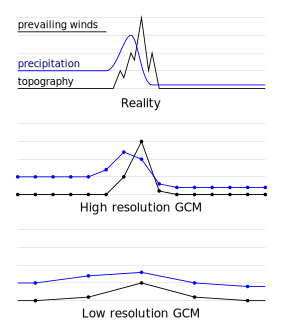
\includegraphics{cordillera-climate-oroprecip}
	\end{center}
	\caption{Schematic representation of the orographic precipitation effect over a mountain range. In a GCM of low resolution, the precipitation peak appears downwind-shifted and smoother and the precipitation shadow is less pronounced than in a high resolution GCM.}
	\label{fig:oroprecip}
\end{figure}

% fig:biatm
\begin{figure*}[t]
	\vspace*{2mm}
	\begin{center}
		\includegraphics{cordillera-climate-biatm}
	\end{center}
	\caption{Ice surface topography (1 km contours) and velocity (\unit{m\,a^{-1}}) after 10\,ka using “hybrid” climate forcing with precipitation rate from WorldClim and surface air temperature from each reanalysis (upper row), and surface air temperature from WorldClim and precipitation rate from each reanalysis (lower row). In other words, the upper row shows the effect of temperature anomalies, and the lower row the effect of precipitation anomalies, for each reanalysis, relative to WorldClim data. Each simulation uses a 5\,\unit{\degree C} offset for comparison with figure~\ref{fig:cool05}}
	\label{fig:biatm}
\end{figure*}

% fig:biatmbars
\begin{figure}[t]
	\vspace*{2mm}
	\begin{center}
		\includegraphics{cordillera-climate-biatmbars}
	\end{center}
	\caption{Effect of temperature and precipitation anomalies (separately and jointly) from each reanalysis on modelled final ice volume relative to the result of the WorldClim 5\,\unit{\degree C} offset simulation. Corresponding ice sheet geometries are presented in figures~\ref{fig:cool05} and~\ref{fig:biatm}}
	\label{fig:biatmbars}
\end{figure}

% fig:best
\begin{figure*}[t]
	\vspace*{2mm}
	\begin{center}
		\includegraphics{cordillera-climate-best}
	\end{center}
	\caption{Ice surface topography (1\,km contours) after 10\,ka using temperature offsets resulting in glaciated areas of circa $2\,\times10^6\,\unit{km^2}$. A reconstructed LGM ice sheet margin by \citet{dyke-2004} (Fig.~\ref{fig:locmap}) is given for reference (blue line).}
	\label{fig:best}
\end{figure*}

% fig:durationstack
\begin{figure}[t]
	\vspace*{2mm}
	\begin{center}
		\includegraphics{cordillera-climate-durationstack}
	\end{center}
	\caption{Left panel: model sensitivity to simulation length. Modelled glaciated area, using NARR forcing data, and temperature offsets from 0 to 15\,\unit{\degree C}, solid lines corresponding to values from 7 to 11\,\unit{\degree C} (left). Right panel: modelled ice margin corresponding to temperature offsets from 7 to 11\,\unit{\degree C} when total glaciated area reach the approximate size of the LGM Cordilleran Ice Sheet of $2\,\times10^6\,\unit{km^2}$. A reconstructed LGM ice sheet margin by \citet{dyke-2004} (Fig.~\ref{fig:locmap}) is given for reference (grey shading). Note that shorter (and colder) simulations lead to more restrictive glaciation of the continental eastern margin but further ice extent in the maritime south-western part of the modelling domain.}
	\label{fig:durationstack}
\end{figure}


% ----------------------------------------------------------------------
\end{document}
% ----------------------------------------------------------------------
